\section{Network Analysis}
As previously mentioned, the friendship network of Yelp is rather incomplete: the majority of users does not have any connections. The users that participate on the social network, however, are highly connected, since $40.92$\% of them are in the large connected component, which means that only $1.80$\% of the OSN participants are absent. The average degree of the whole network is $4.68$ and the clustering coefficient is $0.06$.

Yelp provides an option for users to vote in reviews that they found useful. Figure~\ref{fig:clo_use} relates the closeness centrality to the total useful votes received by a user. We observe that there are roughly three situations: users with low centrality and low usefulness; users with high centrality and low usefulness; and users with high centrality and high usefulness. There is not such a configuration in which users with high usefulness have low centrality. This is a motivation to consider the network structure as an evidence for profile of reviewers.

\begin{figure}[H]
\centering
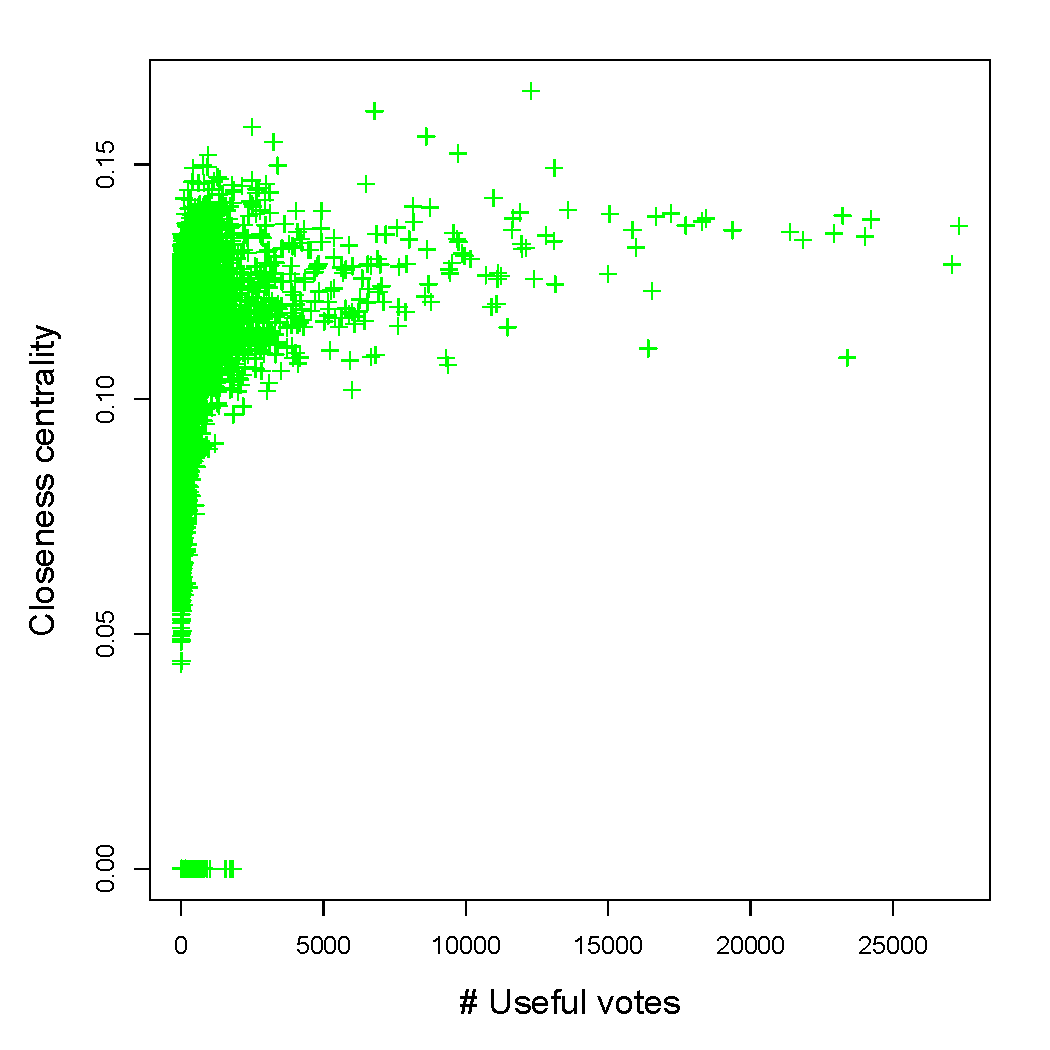
\includegraphics[scale=0.5]{img/close_useful_scatter}
\caption{Correlation between closeness centrality and the number of useful votes for a reviewer.}
\label{fig:clo_use}
\end{figure}

The third set of users cited, a minority, corresponds to reviewers that influence a lot of people. However, few useful votes might indicate that those reviewers provide important experiences for only certain kind of people. Thus, it is necessary to investigate further those reviewers in order to present the information they provide to the ones interested.

\subsection{Homophilly Investigation}

Aiming to validate the presence of homophilly in the network, it was conducted the following experiment: for each edge on the network, the business overlap was computed considering the jaccard similarity of reviewed establishments; a similar process was perfomed for a modified graph with the same nodes and number of edges, which were randomly assigned to pairs. The empirical cumulative distribution of the overlap values are depicted on figure \ref{fig:bus_olap}. We observe a clear difference between the real and the random graphs --- the second practically do not contain positive overlaps, while the first present some.

\begin{figure}[H]
\centering
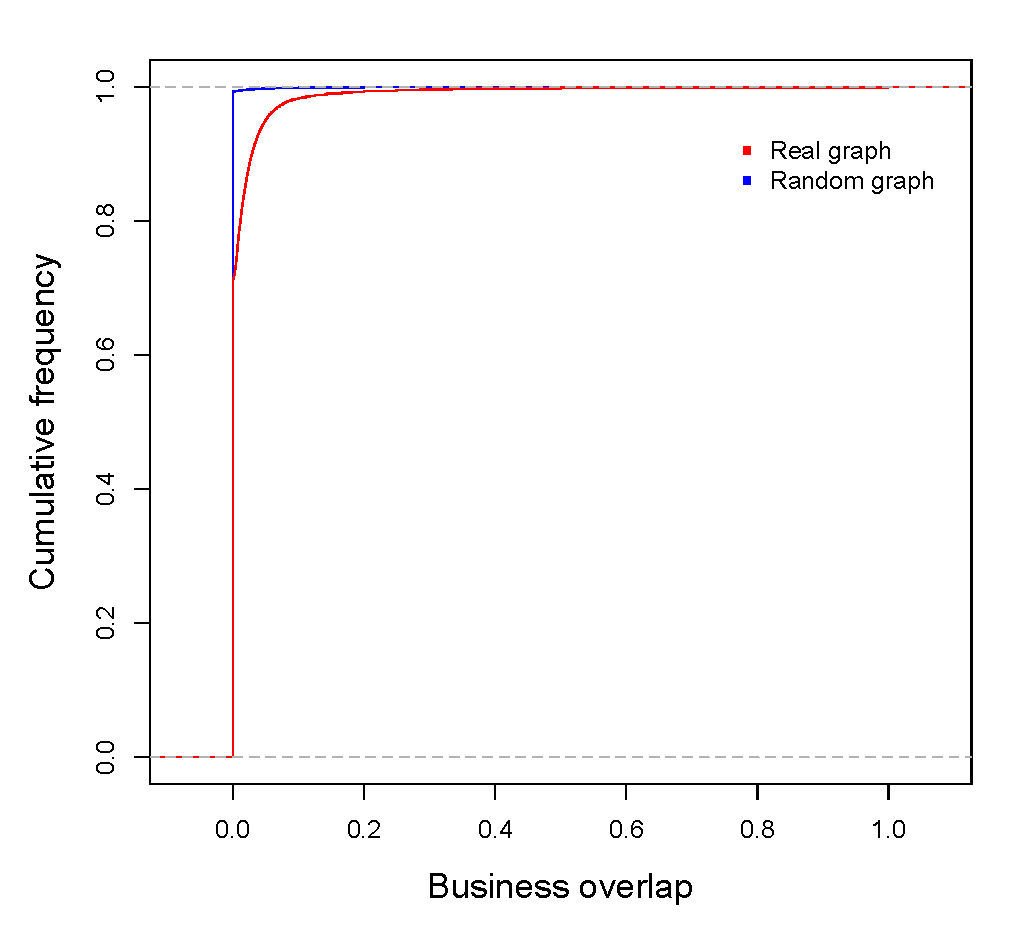
\includegraphics[scale=0.5]{img/ecdf_bus_olap}
\caption{Empirial cumulative distribution of business overlap on real and random graphs.}
\label{fig:bus_olap}
\end{figure}


\subsection{Temporal Effect}
Another important aspect when considering similarity of opinions is the date of
the review. People that visit a place in the same day are more likely to
experience the same events and to have approximate opinions. The figure
\ref{fig:rat_heat} contains the correlation reviews given to the same
stablishment by friends in the same day \ref{fig:fri_eq}, not friends in the
same day \ref{fig:nfri_eq}, friends in different days \ref{fig:fri_dif} and not
friends in different days \ref{fig:nfri_dif}. The results are normalized ---
each cell represents the percentage of co-occurences for the given column. For
example, in figure \ref{fig:fri_eq}, column $1$ has around $40$\% in line
$40$\%. That means that if one individual rates $1$, there is a proportion of
$70$\% of their friends who rated $1$, nearly $30$\% who rated $2$ and
practically $0$\% who rated $3$, $4$ or $5$.

\begin{figure}[H]
  \centering
  \begin{subfigure}[b]{0.5\textwidth}
    \captionsetup{font=small}
    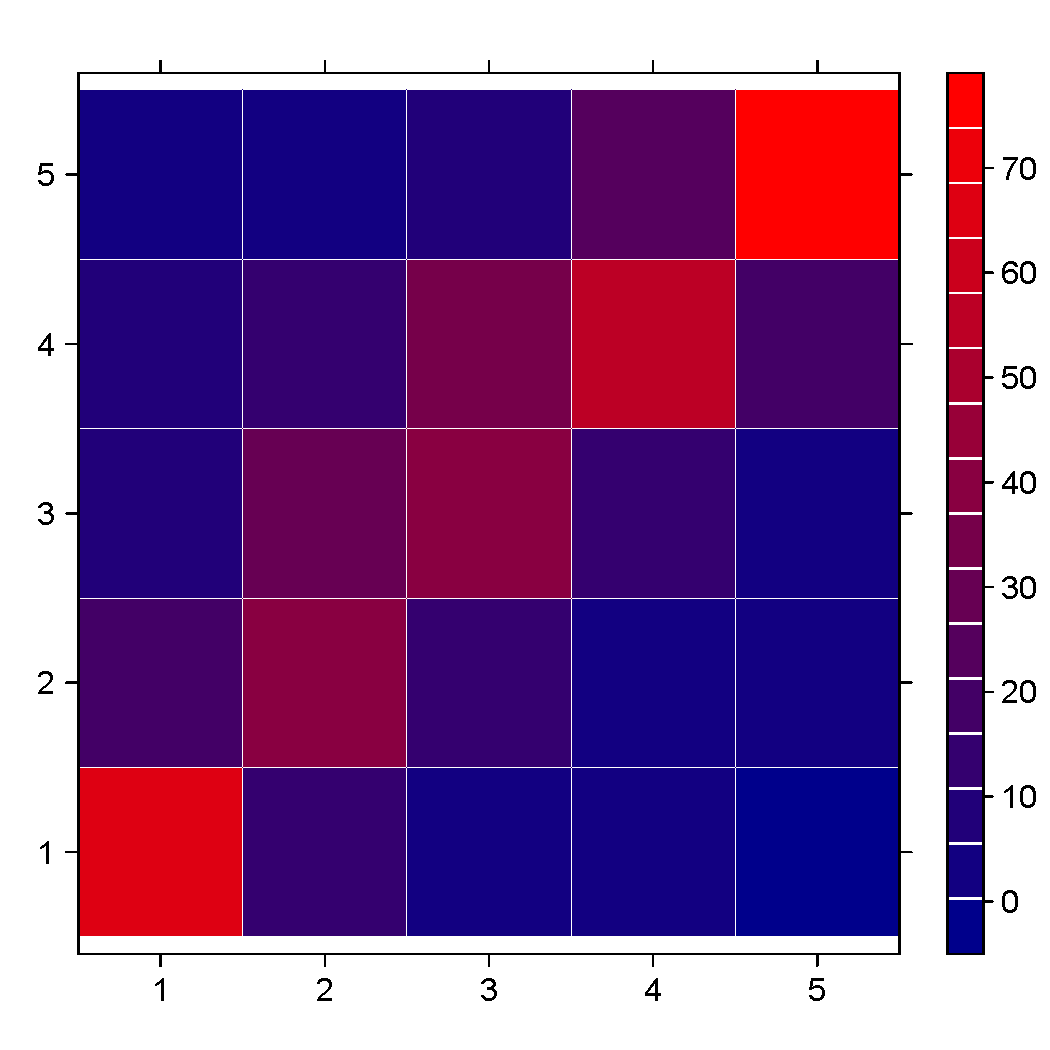
\includegraphics[width=\textwidth]{img/amig_eq_n}
    \caption{Friends in same day.}\label{fig:fri_eq}
  \end{subfigure}%
  ~
  \begin{subfigure}[b]{0.5\textwidth}
    \captionsetup{font=small}
    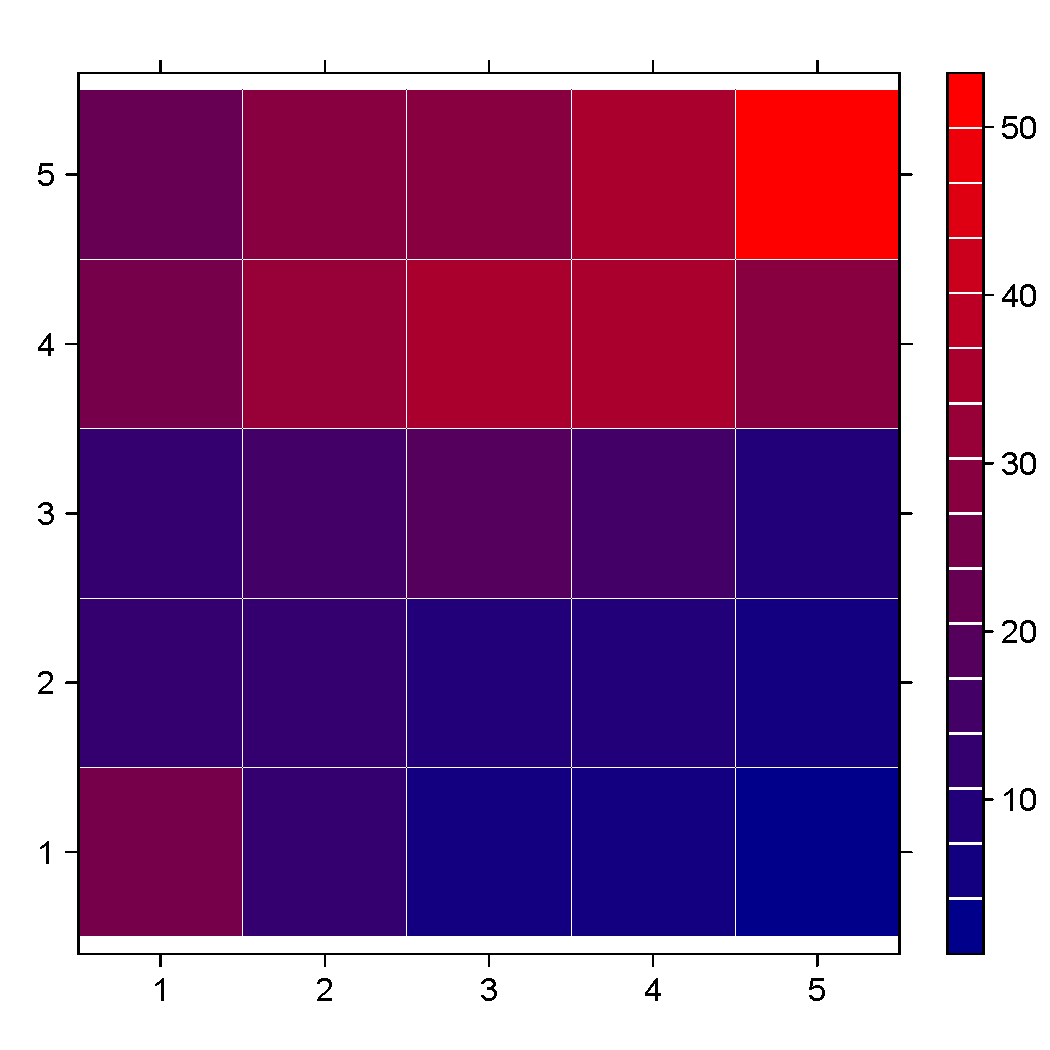
\includegraphics[width=\textwidth]{img/namig_eq_n}
    \caption{Not friends in same day.}\label{fig:nfri_eq}
  \end{subfigure}
  ~
  \begin{subfigure}[b]{0.5\textwidth}
    \captionsetup{font=small}
    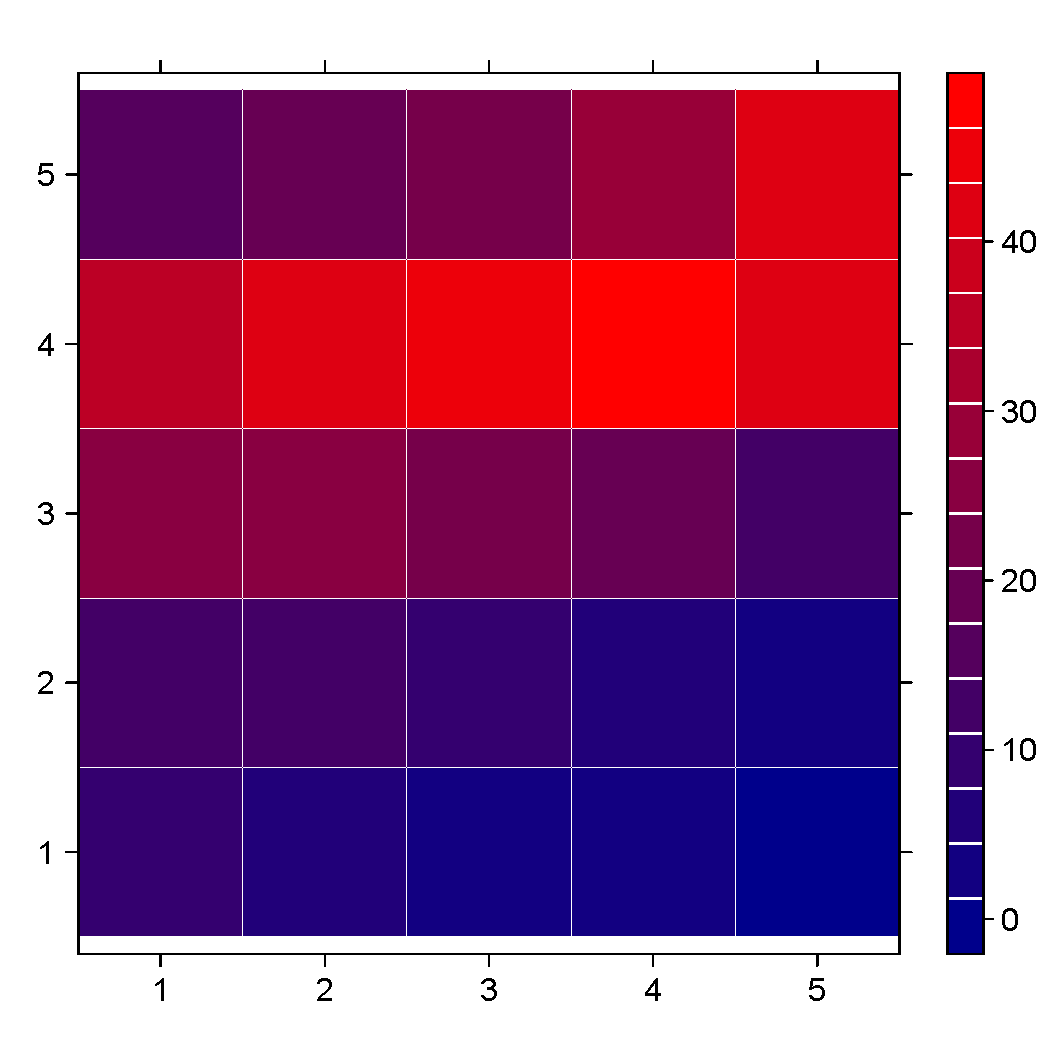
\includegraphics[width=\textwidth]{img/amig_dif_n}
    \caption{Friends in different days.}\label{fig:fri_dif}
  \end{subfigure}%
  ~
  \begin{subfigure}[b]{0.5\textwidth}
    \captionsetup{font=small}
    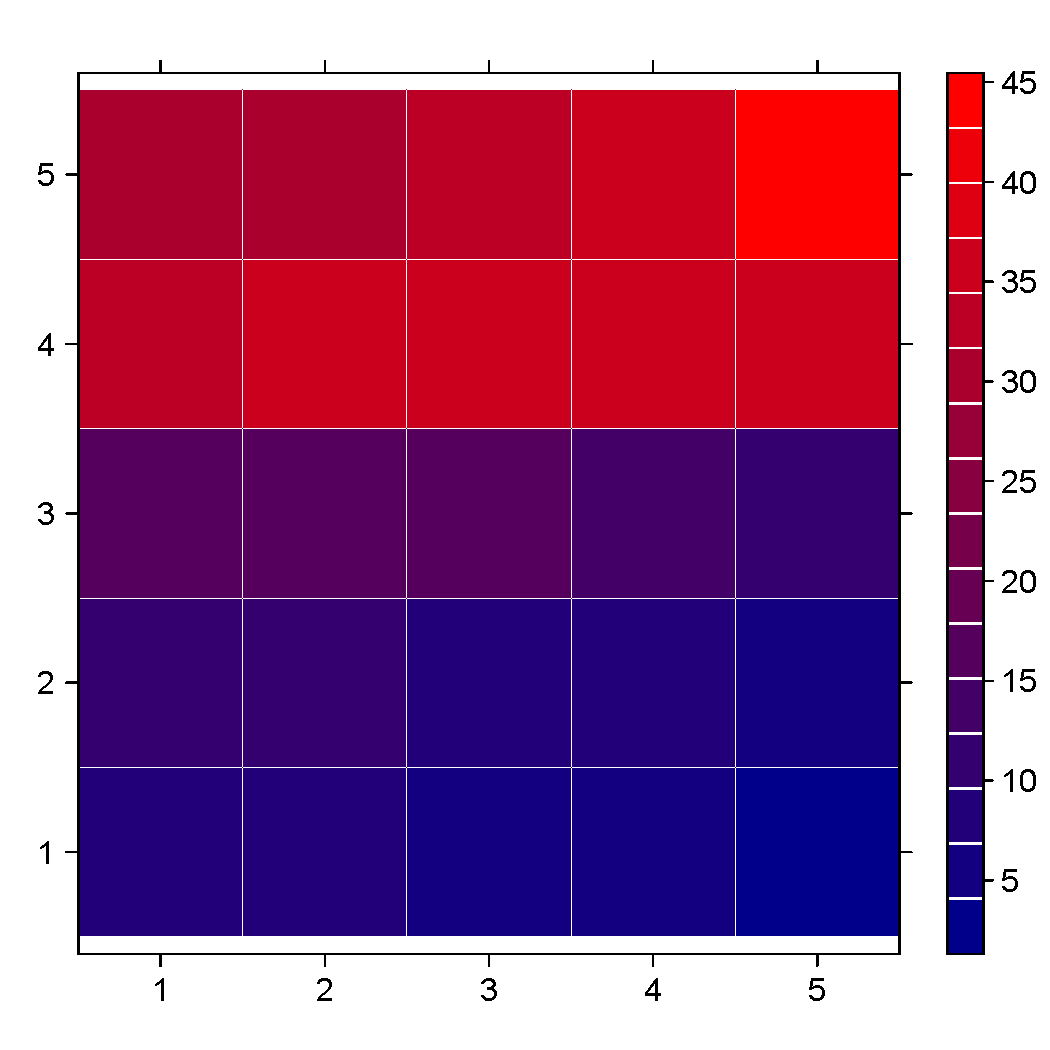
\includegraphics[width=\textwidth]{img/namig_dif_n}
    \caption{Not friends in different days.}\label{fig:nfri_dif}
  \end{subfigure}
  ~
  \caption{Correlation of votes between pair of users percentual by column.}
  \label{fig:rat_heat}
\end{figure}

We can observe a gradative pattern from a strong correlation of ratings to
almost no correlation, in which the proportion of votes on each value rules
the intensity. Another interesting obervation is that there is a greater
agreement between people in the same day than friends in alternative days. This
may be related to the fact that people visiting certain place in the same date
have something in common.

\subsection{Hidden Relationships}
RECAST\cite{} is an algorithm that identifies relationships in dataset of
encounters of people and classifies between friend, bridge, acquaintance and
random. Applying the method for same date reviews, supposing that the day of
the review is the same of the attendance, we obtain the result presented on
table \ref{tab:recast}.

\begin{table}[H]
\begin{tabular}{l|rrrr}
Relationship & \# Friends & \# Bridges & \# Acquaintances & \# Random \\ 
\hline
Friends on Yelp & 69 & 21 & 689 & 634 \\
Not Friends on Yelp & 16 & 3 & 5876 & 13205 \\
\end{tabular}
\caption{Discovered relationships using RECAST.}
\label{tab:recast}
\end{table}

We can observe a great value for acquaintances for Yelp users which are not
friends. This indicates the potential of hidden friends, which share similar
opinions.
